\chapter{Literature Review} % Main chapter title

\label{Chapter2} % For referencing the chapter elsewhere, use \ref{Chapter1} 

\section{All About Research}
Within this chapter we will discuss the research undergone that has helped to reach the conclusion of the overall hypothesis. This will be discussed later on in the chapter. The beginning will be a brief overview and foundation of research, followed by research papers grouped by ideas, a model of processes carried out and the hypothesis of this paper. 
\section{PDDL}
The research undergone for PDDL was based around the language as there are multiple versions that have been released over the years since it was first introduced in 1998 for the first IPC (International Planning Competition) competition\cite{1998IPC}.
\begin{itemize}
\item 1998: STRIPS and ADL
\item 2000: STRIPS and ADL subset
\item 2002: PDDL2.1 Numeric and temporal planning
\item 2004: PDDL2.2 Derived predicates and timed initial literals
\item 2006: PDDL3 Soft goals and trajectory constraints 
\end{itemize}

We have discussed STRIPS and ADL in Chapter \ref{Chapter1}; the next version of PDDL incorporated numeric and temporal planning which was broken down into two subsets, PDDL 2.1 level 2 was the introduction of numeric fluents and PDDL 2.1 level 3 which was level 2 plus action duration. 
Numeric fluents(actions) allows the addition of integers within the conditions of an action\cite{PDDL2.1}. If we need to compare these numeric fluents, it is only possible between other numeric fluents. The effects of an action can be changed in such a way as to incorporate an increase or decrease in these numeric values, for example: 

\begin{verbatim}
(:types bottle)
(:functions
	(amount ?b - bottle
	(capacity ?b - bottle)
		(fluent number))
(:action empty
	:parameters (?b1 ?b2 - bottle)
	:precondition (>= (capacity ?b1) (amount ?b2)
	:effect (and (change (amount ?b1) 0)
	change (amount ?b2)
	(+(amount ?b1)(amount ?b2))
\end{verbatim} 
With this problem we have two bottles and some liquid which we use as the numeric fluent. The goal is to take the liquid from the first bottle and pour it into the second bottle but only if the second bottle has the \textit{capacity} to hold the amount of water from the first bottle. We use the word \textit{change} to update the numeric fluent of each bottle. You can see that the effect of the change in contents from bottle 1 to bottle 2 will result in bottle 1 having the numeric fluent value of \textit{0} as there is no liquid left after the action \textit{empty} has completed. 

A temporal action can be seen as a durative action as a way of modelling the temporal properties of a planning domain\cite{PDDL2.1}. Durative actions can be broken down into discretised and continuous actions. One way it can be expressed is with \textit{duration}. Duration can be applied at the start of an action, in the middle of an action or at the end of an action, so it needs to be placed in the correct area in the domain and should read accordingly. 
\begin{verbatim}
:duration (= ?duration 10)
\end{verbatim}      
An example of the syntax is above and this shows that an action will cost a duration of 10 (could be seconds, minutes, hours etc). 
\\%Check NEW PARAGRAPH INSERTED
\\
The next version of PDDL, PDDL 2.2, was introduced by Stefan Edelkamp and Jorg Hoffman\cite{PDDL2.2}. They created the term \textit{derived predicates} meaning that the predicates do not get effected by the actions. So a set of derivation rules are used instead in the form of:
\\
\\
\textbf{IF}  $\varphi(\overline{x})$  \textbf{THEN}  $P(\overline{x})$\cite{AutomaticPlanning}
\\
\\
\textit{P} is the predicate that can be derived with the vector variable \textit{$\overline{x}$} so then instances of \textit{P} can be true or false. 

Timed initial literals are used to express a restricted form of externally derived events. In other words, at a certain time point in the plan, a fact will become true or false. These times are known to the planner from the beginning in the initial state. As PDDL is moving towards real life events and how to take into account events that do not start out being true but then change as time moves on, using timed initial literals gives that impression. Let's say we have a queue of customers waiting to pay for their shopping with one sales assistant working on a checkout. In the beginning, we have a group of people and one checkout operator. We can say that in the beginning, checkout operator >1 = false. But at some stage, another checkout operator arrives so there are two checkouts now open to serve the customers. Checkout operator >1 has now changed to true. 

PDDL 3 was released in 2006 and introduces the concept of strong and soft constraints on plan trajectories\cite{PDDL3}. The proposition of soft constraints and goals are not required to be completed by the planner to have a valid plan but are more of a desire. A strong constraint or goal requires the planner to satisfy these requirements for a plan to be valid. With regards to soft constraints, a planner should try to satisfy as many of these as possible as it gives better plan quality, however, for strong constraints, these must be met by the planner. The soft constraint aspect can carry a penalty for not satisfying one of these goals/constraints. In other words, when a planner starts to solve a problem in PDDL 3, it must check first for the soft goals/constraints and if not all of them are achievable then the planner must select the costliest subset of soft goals to complete in order to minimise the penalty. This can be extremely difficult as there may be multiple soft goals/constraints that carry different penalty weights and even more so if the planner has a time limit in which to solve the problem. 
There are many ways to express soft and hard goals/constraints but see below as an example:
\begin{verbatim}
(forall (?p - players)
	(preference ScoreGoal
		(sometime (at ?x Score)))
\end{verbatim} 
This could represent a football (soccer) problem where every player on the team must score a goal. This would enforce a penalty for the total number of players that did not score a goal during the plan. We can set this penalty at any cost for each player that did not score. For instance, a striker (forward player) not scoring would have a penalty of 5 because that is his role but a defender would have a penalty of 1 because that is not his role within a game of football.

Now we can look at state trajectories that could be set as soft or strong constraints in the Blocksworld problem.
\\
\\
"Each block should be picked up at least once" 
\begin{verbatim}
(forall (?b - block) (sometime(holding ?b)))
\end{verbatim}\cite{PDDL3} 
This can be set as a hard or soft constraint depending on the requirements of the problem. One way to complete this task for a planner could be to solve the problem with the required blocks by remembering which were used, then pick up the remaining blocks and put them back down after the hard goals/constraints have been satisfied. 

As it is extremely difficult for a planner to incorporate all of the PDDL, in each research paper they use what is called the benchmark for classical planning. This is the recommended set of problems that have been used at the IPC competitions over the past number of years\cite{ICAPS}. For this thesis, STRIPS and ADL have been the choice for testing algorithms and generating results. It will be IPC 1-8, each with 5 domains per ICP, as this will enable fair comparisons to previous work done with STRIPS and ADL to be carried out. 
\section{Classical Planning Algorithms}
In this section, we will discuss the two types of algorithms (forward and backward search) in terms of planning. In state-space planning, we have forward and backward search. In plan space planning we search through a space of partial plans to find a solution. SAT planning turns the problem into a propositional satisfiability problem and given to a SAT solver. Finally we have HTN (Hierarchical Task Network) which is more of an approach rather than a technique of planning, but for this thesis we will focus on state-space planning for classical planning representation. 
\subsection{State-Space Planning}
Within state-space algorithms for planning, the main focus is to create a subset of the state space termed the search space. We can break it down into 3 sub-categories, i.e. each node corresponds to a state of the world, each arc corresponds to a state transition and the current plan corresponds to the current path in the search space\cite{PlanningBook}. We then have three types of algorithm that we can implement for state-space planning: forward search, backward search and a combination of the two. We are able to search in a forward or backward way because of the preconditions and effects. 
\subsubsection{Forward Search}
Best First Search (BFS) is an algorithm that came to light in 2003. The algorithm was developed from the \textit{general search} algorithm described in the book 'Artificial Intelligence: A modern approach'. We can edit this general search algorithm to enforce a best first search algorithm by providing a knowledge area on the queueing function\cite{AModernApproach}. The knowledge gained from the queueing function allows us to determine the next node to be expanded. So the general search algorithm can be easily changed to incorporate a knowledge-type function which evaluates nodes, and the node with the best evaluation is expanded first. 
Once we have the BFS algorithm, we can then incorporate a heuristic function $h(n)$ which estimates the cost of the least expensive path from the state $n$ to the goal state. We use this heuristic function to help select the next node to expand but it is not always the best node overall. When we use a heuristic with BFS, it changes to Greedy Best First Search (GBFS). We consider the algorithm to be susceptible to false starts\cite{StochasticHillClimb}. As an example, say we have a starting node A and we must get to the goal node D. In a tree-like approach, the GBFS algorithm will look for a direct route to the goal and, instead of expanding the two children of A which are B and C, it will only expand one, which could lead the algorithm to a dead end. This means that the algorithm can get stuck and break or we need to introduce a method that will detect repeated states. So if the algorithm goes back to A, it does not go back to B, but instead expands C. 
Another example of how the algorithm works is shown below. In Figure \ref{fig:GBFSTree} the goal is to find the highest cost in the tree, i.e. expand the nodes and generate the highest score.
\\ 
\begin{figure}[!htb]
    \centering
    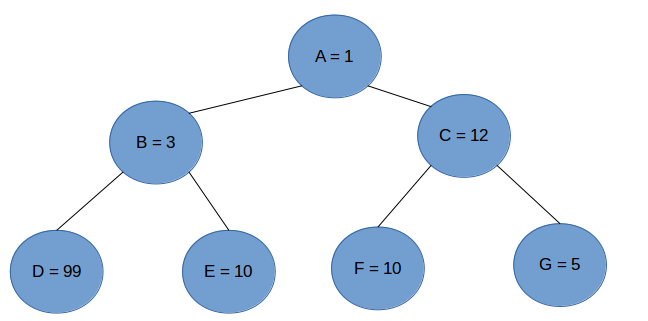
\includegraphics[scale=1.5,width=0.50\textwidth]{GBFSTree.png}
    \caption{GBFS algorithm trying to find the highest score from the nodes}
    \label{fig:GBFSTree}
\end{figure}
\\
The GBFS algorithm will work by selecting the nodes with the highest cost due to the goal that has been set. The algorithm will select \textit{node C} instead of \textit{node B} because 12 is higher than 3. It will then select \textit{node F} because 10 is higher than 5. The algorithm works in such a way that it will never reach the highest scoring node, \textit{node D}. As you can see it works by selecting the optimal immediate choice instead of expanding both nodes \textit{B and C} and checking the successor.
\\
\\
Using a forward search algorithm means that we will start the search from an initial state and use actions within the domain in a certain sequence until a goal state is reached. One of the most popular and well used algorithms that works in a forward search manor is A*. This is the current algorithm implemented in the PDDL4J planner. It was created in 1968 and is an extension to the Dijkstra algorithm\cite{MinimumCostPaths}. As well as being a forward searching algorithm, A* uses heuristics to guide its search towards the goal:

\begin{algorithm}
\caption{A*}
\begin{algorithmic}
\State $openList = set containing start$
\State $closedList = emptySet$
\State $start(g) = 0$
\While {$(openList \textbf{ is not } empty)$}
\State $current = openList(with lowest f cost)$
\If {$current = goal$} 
\State $constructPath(goal)$
\EndIf
\State $remove(current) \textbf{ from } openList$
\For {$eachNeighbour \in currentNeighbour$}
\If {$neighbour \textbf{ is not in } closedList$}
\State $add(neighbour)$
\Else { $openNeighbour = neighbour \in openList$}
\EndIf
\If {$neighbour = neighbour \in openList$}
\State $openNeighbour(g) = neighbour(g)$
\State $openNeighbour(parent) = neighbour(parent)$
\EndIf
\EndFor
\EndWhile
\end{algorithmic}
\end{algorithm}

We will look closely at this algorithm (see Algorithm 1 above) and the use of the weight functions $f(n) = g(n) + h(n)$. This essentially is the use of two types of algorithms, Best First Search and Dijkstra. If $h(n) = 0$ then $f(n)$ becomes $g(n)$ which is Dijkstra's shortest path algorithm. If $h(n) = \textit{large number}$ then $g(n)$ is ignored and it becomes Best First Search. So the use of an admissible heuristic with A* helps to balance out the two functions that make $f(n)$ which in turn creates a direct shortest path algorithm.\cite{InformedSearch}
From this we can see that A* is realistically more of a method than a point A to point B algorithm. Overall, it is a container for a greedy algorithm combined with a heuristic search function.  
\\
\\
Enforced Hill Climbing (EHC) is an algorithm that was implemented in a famous planner called Fast Forward (FF) \cite{FFPlanner}. EHC is an updated version of a generic hill-climbing algorithm. Hill climbing is used in mathematical optimisation in the area of local search. The main function in hill climbing is that it starts with an arbitrary solution and iteratively changes a single element in the original solution; if the new solution is better than the old then the old is replaced and the algorithm will continue to do this until no changes occur in the newest solution. 
Regarding EHC, what we want to achieve is a sequence of actions that in turn leads to a better successor if, at that moment, none are present. One of the main issues with EHC is that, with a heuristic to guide the search, EHC can get stuck in a dead-end or be unable to escape a plateau, meaning that within the search space, the heuristic values of all successors are greater than or equal to the best nodes already explored\cite{PlateauEHC}. What we would want to achieve when using EHC is to provide a method to escape the algorithm being stuck and never finding a solution within a specified time limit. 
\\ 
\begin{algorithm}
\caption{Enforced Hill Climbing}
\begin{algorithmic}
\State $openList = initialState$
\State $bestHeuristic = heuristicValue(initialState)$
\While {$(openList \textbf{ is not } empty)$}
\State $currentState = pop state \textbf{ from } head of openList$ 
\State $ successors = the list of states visible from currentState$ 
\While {$ successors \textbf{ is not } empty$}
\State $nextState = remove a state \textbf{ from } successors$
\State $h = heursticValue(nextState)$
\If {$nextState = goalState$}
\State $return(nextState)$
\EndIf
\If{$h is better than best heuristic$}
\State $clear(successors)$
\State $clear(openList)$
\State $bestHeuristic = h$
\EndIf
\State $place next state at back of open list$
\EndWhile
\EndWhile
\end{algorithmic}
\end{algorithm}
\\
In algorithm 2 above, we can see the comparison of the heuristic function $h$ and whether it is better than the best heuristic function available. 
\subsubsection{Backward Search}
A backward search algorithm does exactly what you would expect in that it works in the opposite way to a forward search algorithm by starting from a goal state and using actions in a certain sequence until an initial state is reached. 
There are many algorithms like A* and Dijkstra that can be used for forward search or backward search.
\\ 
\begin{algorithm}
\caption{DIJKSTRA}
\begin{algorithmic}
\State $dist[s] \leftarrow 0 $
\ForAll {$v \in V-(s)}$
\State $ dist[v] \leftarrow \infty$
\EndFor
\State $S \leftarrow 0$
\State $Q \leftarrow V$
\While {$Q \neq 0$}
\State $ u \leftarrow minDistance(Q, dist)$ 
\State $S \leftarrow S \cup (u)$
\ForAll {$v \in neighbours[u]$}
\If {$dist[v] > dist[u] + w(u, v)$}
\State $d[v] \leftarrow d[u] + w(u, v)$
\EndIf
\EndFor
\EndWhile
\State $return(dist)$
\end{algorithmic}
\end{algorithm}
\\
The distance to source is marked as 0 and we set all others to infinity. We then select the elements of $Q$ with the minimum distance and add $u$ to the list of visited vertices. Following this, we perform a check to see if a new shortest path can be found. If so, set the new shortest path value and return the distance. 
Dijkstra performed in a backward search will use the same approach and vertices with each arc $w(u, v)$ becomes $w(v, u)$ (see algorithm 3).
\section{SAT and SAT4J} 
SAT4J takes in files of CNF format as explained in Chapter \ref{Chapter1}. SAT4J is a Java library for solving boolean satisfiability and optimization problems\cite{SATandSAT4J}. It is able to solve a range of different types of problems and its written in Java. It is open source and uses a pseudo-boolean solver as a universal engine which translates the problems\cite{SATandSAT4J}. 

\begin{figure}[!htb]
    \centering
    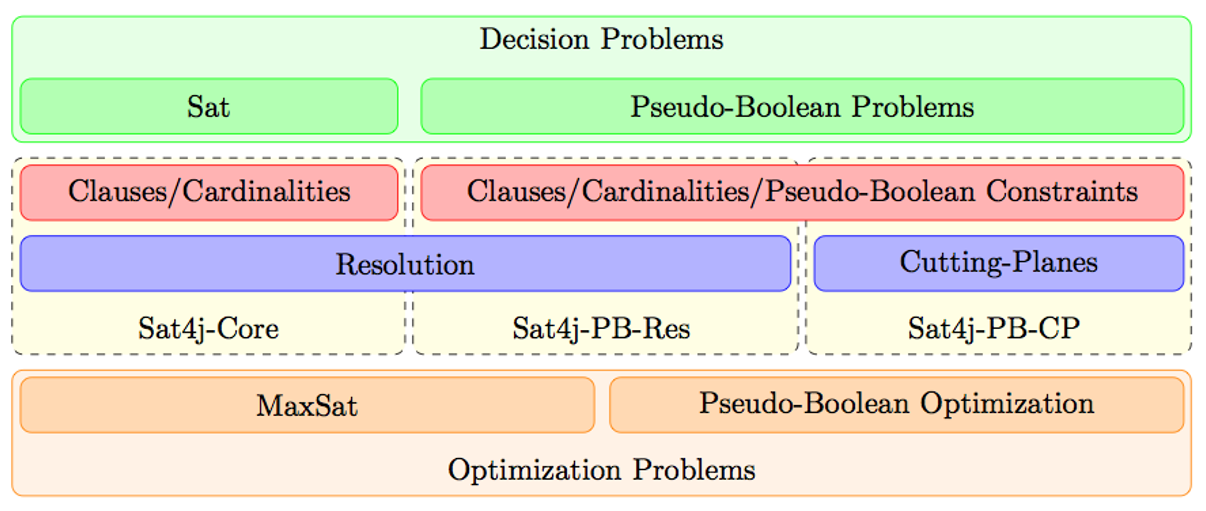
\includegraphics[scale=0.27]{SATFeaturesNew.png}
    \caption{Overview of the SAT4J features}
    \label{fig:SAT4J}
\end{figure}
In Figure \ref{fig:SAT4J} you can see an overview of the SAT4J system\cite{SATandSAT4J}. SAT was the first problem within the planning domain to be NP-complete based on the Stephen Cook theorem\cite{SteveCook}. NP represents for Non-deterministic Polynomial time and NP-complete means that any problem can be solved in polynomial time using a non-deterministic Turing machine. This is a theoretical concept in the field of computer science.
Below we show the basic semantic for a CNF file. 
If we have a formula:
\begin{verbatim}
(p(1) OR (NOT p(3)))
AND
(p(2) OR (p(3) OR (NOT p(1)))
\end{verbatim}
we can convert this into CNF format like so:
\begin{verbatim}
p cnf 3 2
1 -3 0
2 3 -1 0
\end{verbatim}
The first line \textit{p cnf 3 2} means that this is the first line of the problem; it is in conjunctive normal form; and there are 3 variables and 2 clauses. The next lines below are the clauses and they finish with a \textit{0} to let the solver know that the clause has finished. We represent \textit{OR} by a space in the clause and an \textit{AND} with a new line as seen above.
The SAT solver will then decide if this problem is satisfiable (or not) depending on the input by the user.
\begin{verbatim}
c 2 constraints processed
s SATISFIABLE
v -1 -2 -3 0
c Total wall clock time (in seconds) : 0.023 
\end{verbatim}
\textit{(The 0 at the end has been outputted to show the end of the clause)}
\\% CHECK PARAGRAPH
\\
We can see from the above output that the problem was satisfiable in a total time of 0.023 seconds. Translating it back to logic it looks like this:
\begin{verbatim}
(NOT p(1) OR p(2) OR p(3)
\end{verbatim} 
 
\section{Heuristics}
As discussed in Chapter \ref{Chapter1}, a heuristic function will involve a relaxed version of the problem. In some heuristics, the plan is to relax the problem so that a small subset of it can be solved so it makes it less computationally expensive to solve a problem. When the planning problem is relaxed, the deleted list of actions is ignored. These are the negative effects of an action.\cite{IgnoringDeleteLists} 
\begin{verbatim}
  (:action put-down
	     :precondition (holding ?x)
	     :effect
	     (and (not (holding ?x))
\end{verbatim} 
Taking a look at this example above shows how, within PDDL, the negative effect of an action is coded within the domain but, with heuristic functions, we ignore these notations of $and(not(xxxx)$ for negative effects as they provide no help to the state of the environment.
The area of heuristics can be broken down into 2 categories: admissible and not admissible. An admissible heuristic $h$ for all $s \in S: h(s) \leq h^*(s)$. This will mean that it does not overestimate the distance to the goal node. Not admissible heuristics can over-estimate or underestimate the distance to the goal node. 
In the PDDL4J library there are a number of heuristics that have already been implemented; the table below shows a list of heuristics and if there are admissible or not admissible.
\begin{center}
  \begin{tabular}{ | l | p{3cm} | l |}
    \hline
    \textbf{Heuristics} & \textbf{Method} & \textbf{Admissible/Not Admissible} \\ \hline
    Adjusted Sum & $sum(cost(pi)) + delta(S)$ & Not Admissible  \\ \hline
    Adjusted Sum 2 & $cost(S) + delta(S)$ & Not Admissible  \\ \hline
    Adjusted Sum 2M & $cost(S) + delta(S)$ with mutex& Not Admissible  \\ \hline
    Combo & $sumheuristic(S) + setlevel(S)$& Not Admissible  \\ \hline
    Fast Forward & Uses a relaxed graph to ignore negative effects & Not Admissible  \\ \hline
    Set Level & Return the level of the planning graph where all propositions of the goal are & Admissible \\ \hline
    Sum & Sum all the individual costs of each action &Not Admissible \\ \hline
    Sum Mutex & Sum heuristic where mutual exclusions are computed & Not Admissible \\ \hline
    Max & Calculates the most expensive atom & Admissible \\ 
    \hline
  \end{tabular}
\end{center}
As there are multiple heuristics implemented within the PDDL4J planer, I will explain briefly a not admissible heuristic Sum and how it can be changed with one line to make it the Max heuristic which is admissible. 
\subsection{Sum $H^+$}
This heuristic function is called $h_0(s)$, otherwise known as the sum algorithm.
\begin{equation}
\begin{aligned}
Delta(s)\\
  & \textbf{for each } p \textbf{ do}: if p \in s \textbf{ then } \triangle_0 (s,p) \leftarrow 0 \\
  & else \triangle_0 (s,p) \leftarrow \infty \\
  & U \leftarrow {s}\\
  & Iterate\\
  & \textbf{for each } a \textbf{ such that } \exists u \in U, precond(a) \subseteq u \textbf{do}\\
  & U \leftarrow {u} \cup effects^+(a)\\
  & \textbf{ for each } p \in effects^+(a) \textbf{ do}\\
  & \triangle_0 (s,p) \leftarrow min {\triangle_0 (s,p), cost(a) + \sum q \leq precond(a) \triangle_0 (s,q)}
\end{aligned}
\end{equation}
We set the costs of the propositions appearing in the initial state as 0 and the cost of the rest $\infty$. We then update the costs until a fixed point is reached. So if we have a planning problem and each action has a $cost(a)$, we can try to estimate the distance to a proposition $p$ or $g$. We do this by summing all the individual costs of each action.\cite{PlanningGraphs} If there is a solution to the problem, the sum algorithm will achieve it in polynomial time. Although it is a very informative heuristic, it is not admissible. 
\subsection{Max $H^1$}
Max is a popular heuristic but is not widely used in planning competitions because, for any given state, max calculates the most expensive atom in the state. It works by considering a relaxed version of the problem. 
The max algorithm is the same as the sum algorithm except for one line.\cite{PlanningBook} The \textit{for} loop for the positive effects changes to:
\begin{equation}
\triangle_1 (s,p) \leftarrow min{ \triangle_1 (s,p), 1 + max{\triangle_1 (s,q) | q \in precond(a)}}
\end{equation}
The max heuristic is not as informative as other heuristics as it computes the most costly sub-goals. 

\section{State of the Art}
The best way to view state of the art in state-space planning is the International Conference on Automated Planning and Scheduling, otherwise known as the International Planning Competition (IPC) \cite{ICAPS}. This competition is for planners to be tested against others on different domains and problems. The competition has been running since 1998 and uses different domains each time that are submitted by teams incorporating different levels of PDDL. For each of the conferences there have been new PDDL additions as discussed earlier. 
The competition breaks the planners down into sub-categories.
\begin{itemize}
\item Deterministic part 
\item Learning part
\item Probabilistic part
\end{itemize}
Within each of these sub-sections are domains and problems that correlate to a specific task as it is difficult for all planners to be able to participate in all events. In this thesis, the deterministic section will be the main focus. 
\subsection{Search Algorithms and Heuristics}
Looking at a number of planners that participated in the IPC competition over the past years, A* has been used various times as the main search algorithm but has been incorporated with other search algorithms to give a better overall search. A main algorithm used is one designed by Malte Helmert for the Fast Downward planner\cite{FastDownward}. It is based upon the FF (Fast Forward) planner that was designed by Jorg Hoffmann and Bernhard Nebel.\cite{FFPlanner} The FF planner won the IPC competition in 2000 and is based upon two functions: a search algorithm called Enforced Hill Climbing with a Best First Search as its "back-up" search function, and a heuristic function called Graphplan. Figure \ref{fig:FFplanner} shows the system architecture for the FF planner; the heuristic Graphplan is called at every state by the EHC algorithm and it is a forward search planner.
 
\begin{figure}[!htb]
    \centering
    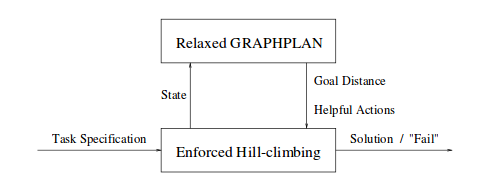
\includegraphics[scale=0.7]{FFplanner.png}
    \caption{System architecture for the FF planner}
    \label{fig:FFplanner}
\end{figure}

Fundamentally, it uses the EHC algorithm to find a solution to a problem but, as the algorithm is susceptible to getting stuck in dead ends as pointed out in \cite{FFPlanner}, there is a complete heuristic search engine built into FF that will start from the beginning if EHC fails, which helps to guarantee a solution. As well as the heuristic function, it has a backup algorithm Best First Search – and all of these functions together help build a very sound planner.  

Fast Downward is based on this approach and it was the winner of the IPC competition in 2004 \cite{IPC2004W}. It is constructed in the same way as FF as it is a heuristic search planner but it uses a different heuristic function called Casual Graph Heuristic. This heuristic approximates goal distances by solving a hierarchy of local planning problems \cite{CasualGraph}; these problems only include a single state variable and the dependant variable. Within a casual graph we think of nodes as the variables in the problem and the links within the graph show the dependencies among the variables. The estimate that it provides is the number of operators needed to reach the goal from a state $s$ in terms of estimated costs of changing the value of each variable $v$ that appears in the goal from its value $s(v)$ in $s$ to its value $s_*(v)$ in the goal.\cite{CasualGraph}
Malte Helmert and Hector Geffner describe the casual graph estimate function as:
\begin{equation}
h(s) = \sum_{v\in dom(s_*)} cost_v(s(v), s_*(v))
\end{equation}
The Fast Downward planner incorporates two actual search algorithms to create a plan. It uses a Greedy Best First Search (GBFS) with the casual graph heuristic, and the second is multi-heuristic BFS which combines different heuristic evaluators. The workings of the GBFS have been discussed earlier.
The multi-heuristic BFS works in a very simple way in that it will use multiple heuristics to direct the search towards a common goal. The idea behind it is that the heuristics will hopefully complement each other by having different weaknesses. So if one heuristic gets stuck in one section of the plan, the other heuristic may be able to find a solution for that particular problem efficiently and quickly and, therefore, negating the possibility of plateaus. But instead of combining the heuristic estimates into a single value, each heuristic alternates expanding a state from each open list.\cite{FastDownward}

Fast Downward uses a combination of a Casual Graph Heuristic and a Fast Forward heuristic (FF). The documentation for the Fast Downward planner \cite{FDownwardDoc} explains that both the Casual Graph heuristic and the FF are not admissible. From work previously carried out, a heuristic is not admissible when it may overestimate optimal costs.\cite{Pearl}\cite{Nilson} \cite{AdmissibleHeuristic} This shows that the Fast Downward planner in this sense is not optimal because it uses heuristics that are not admissible. Overall it means that when using these heuristics combined with the multi-heuristic BFS algorithm, the plans found are not optimal in terms of steps taken to achieve a goal. 
In the most recent IPC competition, the first-place planner in the deterministic track, the basis was Fast Downward and FF so we can see that using these algorithms provides non-optimal plans but this is sacrificed for speed and memory consumption, as well as solving problems. 

One of the main heuristics used by multiple planners is the Fast Forward heuristic, developed by Hoffmann and Nebel\cite{FFPlanningSystem}. Its main function is that from a current state, it finds a relaxed version of the problem and also ignores the negative effects from actions. The basis of the Fast Forward heuristic is that it uses a relaxed version of GraphPlan to compute the heuristic value. 

The algorithms over the years have not changed much but the heuristic functions have changed drastically. The PDDL4J planner has optimal heuristic functions that can be used with the A* search algorithm but A* is only an optimal search algorithm if the heuristic is admissible. 

From the two main planners we looked at in this section, the FF planner attempted 284 problems in the IPC 2002 competition and successfully completed 237 of them, giving it an 83\% success rate. The Arvanherd planner, the winner of the IPC 2014 competition, was built upon the Fast Downward planner and uses the FF heuristic. It was able to solve a total of 161 problems\cite{ArvandHerd}. The total success rate is unknown for Fast Downward.  
\section{Hypotheses}
In this section we will define the hypothesis for this thesis. Based within the PDDL4J library, there is reason to believe that the A* algorithm is not as optimal as other search algorithms. Yes, provided with the correct heuristic, it provides an optimal plan but is it optimal in terms of speed and memory consumption? Also, are the heuristics within the planner optimal in terms of plan size and are they truly admissible or not?

As stated in the previous section, there are other search algorithms and heuristics that provide fast and efficient results for classical planning problems. The goal is to implement a new search algorithm for the PDDL4J planner based on the research conducted and also a new heuristic. The PDDL4J library will be tested against the new algorithm and heuristic as well as tested against other planners from the IPC competition.

The last part of the thesis will show how a different area of planning can complete classical planning tasks. We will use the SAT4J library to run classical planning tasks and compare the results from the SAT4J library to the results from the PDDL4J library to see if satisfiability problems are easier to solve than classical planning approaches using PDDL.  
